\documentclass{article} % For LaTeX2e
\usepackage{iclr2026_conference,times}

% Optional math commands from https://github.com/goodfeli/dlbook_notation.
\input{math_commands.tex}

\usepackage{hyperref}
\usepackage{url}

\usepackage{natbib}
\usepackage{algorithm}
\usepackage{algorithmic}

% Mathematical packages
\usepackage{amsmath}
\usepackage{amssymb}
\usepackage{amsthm}
\usepackage{mathtools}
\newtheorem{definition}{Definition}[section]

\usepackage{amsthm}
\usepackage{enumitem}
\usepackage{tikz}
\usepackage{multirow}
\usepackage{caption}
\usepackage{subcaption}
\usepackage{booktabs}
\usepackage[table]{xcolor}

\usepackage{pgfplots}
\pgfplotsset{compat=1.18} % or any recent version



\title{Markovian Transformers for Informative Language Modeling}

% Authors must not appear in the submitted version. They should be hidden
% as long as the \iclrfinalcopy macro remains commented out below.
% Non-anonymous submissions will be rejected without review.
% \iclrfinalcopy
\author{Scott W. Viteri, Max Lamparth, Peter Chatain \& Clark Barrett \\
Department of Computer Science\\
Stanford University\\
Stanford, CA 94305, USA \\
\texttt{\{sviteri,lamparth,pchatain,barrettc\}@stanford.edu}
}

% The \author macro works with any number of authors. There are two commands
% used to separate the names and addresses of multiple authors: \And and \AND.
%
% Using \And between authors leaves it to \LaTeX{} to determine where to break
% the lines. Using \AND forces a linebreak at that point. So, if \LaTeX{}
% puts 3 of 4 authors names on the first line, and the last on the second
% line, try using \AND instead of \And before the third author name.

\newcommand{\fix}{\marginpar{FIX}}
\newcommand{\new}{\marginpar{NEW}}

%\iclrfinalcopy % Uncomment for camera-ready version, but NOT for submission.
\begin{document}


\maketitle
\begin{abstract}
Chain-of-Thought (CoT) reasoning often fails to faithfully reflect a language model's underlying decision process. We address this by introducing a \emph{Markovian} language model framework that can be understood as a reasoning autoencoder: it creates a text-based bottleneck where CoT serves as an intermediate representation, forcing the model to compress essential reasoning into interpretable text before making predictions. We train this system with a GRPO-style policy gradient algorithm using parallel sampling, a frozen baseline CoT$'$, within-batch standardized advantages, and actor-reward (chain-rule) gradients. On QA tasks, Markovian training recovers most of the gains of a non-Markovian GRPO variant while forcing the model to answer from the CoT alone (e.g., GSM8K: 19.6\% $\to$ 57.1\%; ARC-Challenge: 36.1\% $\to$ 79.9\%; on average only $\approx$3--4 pp below a non-Markovian upper bound). Perturbation analyses across types and severities show that Markovian models incur systematically larger log-probability drops under CoT corruption than matched Non-Markovian baselines, indicating stronger causal reliance on the CoT. Cross-model evaluation confirms that learned CoTs generalize across architectures, suggesting they capture transferable reasoning patterns rather than model-specific artifacts.
\end{abstract}

\section{Introduction}
\label{sec:intro}
The rapid advancement of language models (LMs) has led to impressive performance on complex cognitive tasks~\citep{NEURIPS2020_1457c0d6}. Yet it is often unclear \emph{why} an LM arrives at a particular conclusion~\citep{lamparth2023analyzing,burns2024discovering,gurnee2024language}, causing issues in high-stakes applications~\citep{Grabb2024.04.07.24305462,lamparth2024human,rivera2024escalation}. Traditional interpretability methods analyze hidden activations or attention patterns to extract ``explanations''~\citep{geiger2022inducing,geva2022transformer,meng2022locating,raukur2022toward,wang2022interpretability,lamparth2023analyzing,nanda2023progress}. Modern LMs, however, already generate coherent text: we might hope \emph{prompting} the model to articulate its reasoning (``Chain-of-Thought'' or CoT)~\citep{nye2022show,wei2022chain} would yield a faithful record of its thought process. 

Unfortunately, CoT explanations can be \emph{unfaithful}. For example, \citet{turpin2023language} show that spurious in-context biases often remain hidden in the CoT, and \citet{lanham2023measuring} find that altering CoT text may not affect the final answer. Such observations indicate that standard CoTs are not ``load-bearing.''

In this work, we take a \emph{pragmatic} approach to interpretability, focusing on \emph{informativeness} over full faithfulness. Rather than insisting the CoT mirrors the model's entire internal process, we require that \emph{the CoT alone suffices to produce the final answer}. In other words, if we remove the original prompt and rely only on the CoT, the model should still reach the correct output. This makes the CoT \emph{causally essential} and \emph{fragile}: changing it necessarily alters the prediction.

What distinguishes our approach is the clear distinction between the model \emph{relying on its CoT} versus generating \emph{more informative CoTs}. While traditional approaches train models to generate better-quality CoTs, they don't fundamentally change how the model uses them. Our Markovian framework, by contrast, forces the model to process information through the CoT bottleneck, making the CoT not just informative but \emph{causally load-bearing} for prediction.

For instance, Llama's CoT on arithmetic tasks changed dramatically after training. \textbf{Before training}, it simply listed all numbers and their (incorrect) sum (e.g., ``Sum = 76 + 90 + 92 + ... = 2314''). \textbf{After training}, it performed correct step-by-step calculations (e.g., ``calculate 6 + 89 = 95; Next, calculate 95 + 38 = 133...''), breaking the task into manageable steps that can be verified independently and enabling accurate answer prediction even when the original question is removed.

\paragraph{Recipient-Specific Compression.}
A key insight is that an \emph{informative} CoT can also serve as a \emph{recipient-specific compression} of the model's hidden knowledge: it distills the essential reasoning into text that another recipient (e.g.\ a different model or a human) can use to predict the same outcome. Our experiments confirm that the learned CoTs generalize across interpreters, suggesting that these textual explanations genuinely encode transferable problem-solving steps rather than model-specific quirks (Section~\ref{subsec:interp}).

\paragraph{Contributions.}
\begin{enumerate}
    \item We introduce a Markovian language model framework that structurally enforces CoT generation to be causally essential, together with a GRPO-style training recipe (parallel sampling, frozen CoT baseline, actor-reward gradients) that optimizes this objective through a discrete text bottleneck.
    \item We apply this framework to arithmetic problems (Mistral 7B) and standard QA datasets (GSM8K, MMLU, SVAMP, ARC-Challenge; Llama 3.1 8B), observing large absolute gains over the base model (e.g., GSM8K 19.6\% $\to$ 57.1\%, ARC-Challenge 36.1\% $\to$ 79.9\%) while remaining within $\approx$3--4 percentage points of a Non-Markovian GRPO variant that can still see the question during answer prediction.
    \item We show through systematic perturbation analyses on Wikipedia continuation and multiple QA datasets that Markovian training produces consistently higher sensitivity to CoT perturbations compared to matched Non-Markovian baselines (Tables~\ref{tab:markovian_comparison} and~\ref{tab:qa_fragility_detailed}), indicating that the learned CoTs are more causally load-bearing.
    \item We demonstrate cross-model transfer: CoTs trained on one model (Llama 3.1 8B) remain informative for diverse other models (Mistral, Phi, Qwen, GPT-2) on GSM8K and Wikipedia. This underscores the CoT's \emph{recipient-specific} informativeness and suggests it captures a shared reasoning strategy rather than model-specific artifacts.
\end{enumerate}

Section~\ref{sec:related_work} reviews related work, Section~\ref{sec:MLM} details our Markovian framework, and Section~\ref{sec:method} describes the RL training. Section~\ref{sec:experiments} presents empirical results, and Section~\ref{sec:disc} discusses limitations and future directions.


\begin{figure*}[t!]
  \centering
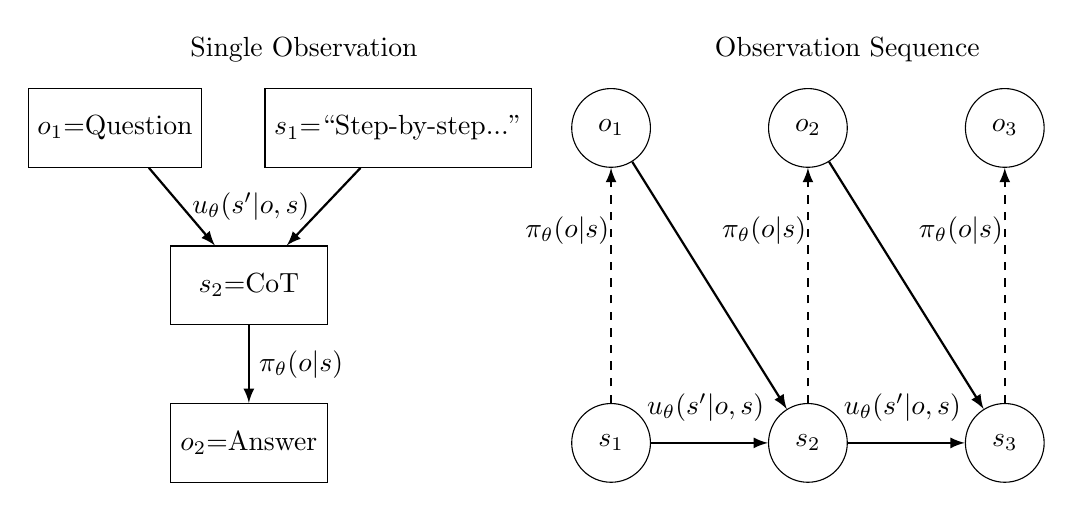
\begin{tikzpicture}[
    node distance=2cm,
    box/.style={rectangle, draw, minimum width=2cm, minimum height=1cm},
    circlebox/.style={circle, draw, minimum size=1cm},
    arrow/.style={->, thick},
    >=latex
]

% Left side: Single timestep
\node[box] (Q) at (-4.3,2) {$o_1$=Question};
\node[box] (S) at (-0.7,2) {$s_1$=``Step-by-step...''};
\node[box] (CoT) at (-2.6,0) {$s_2$=CoT};
\node[box] (A) at (-2.6,-2) {$o_2$=Answer};

\draw[arrow] (Q) -- node[right] {$u_\theta(s'|o,s)$} (CoT);
\draw[arrow] (S) -- (CoT);
\draw[arrow] (CoT) -- node[right] {$\pi_\theta(o|s)$} (A);

% Right side: Causal structure
% Observations
\node[circlebox] (o1) at (2,2) {$o_1$};
\node[circlebox] (o2) at (4.5,2) {$o_2$};
\node[circlebox] (o3) at (7,2) {$o_3$};

% States
\node[circlebox] (s1) at (2,-2) {$s_1$};
\node[circlebox] (s2) at (4.5,-2) {$s_2$};
\node[circlebox] (s3) at (7,-2) {$s_3$};

% Connections
\draw[arrow] (o1) to (s2);
\draw[arrow] (s1) to (s2);
\node[above] at (3.2,-1.85) {$u_\theta(s'|o,s)$};

\draw[arrow] (o2) to (s3);
\draw[arrow] (s2) to (s3);
\node[above] at (5.7,-1.85) {$u_\theta(s'|o,s)$};

% π(o|s) connections
\draw[arrow, dashed] (s1) to (o1);
\node[left] at (2.1,0.7) {$\pi_\theta(o|s)$};

\draw[arrow, dashed] (s2) to (o2);
\node[left] at (4.6,0.7) {$\pi_\theta(o|s)$};

\draw[arrow, dashed] (s3) to (o3);
\node[left] at (7.1,0.7) {$\pi_\theta(o|s)$};

% Labels
\node at (-1.9,3) {Single Observation};
\node at (5,3) {Observation Sequence};

\end{tikzpicture}
\caption{Markovian training as a reasoning autoencoder. Left: Single time-step process from Question to CoT to Answer, creating a text-based bottleneck where the CoT must capture all information needed for answer prediction. Right: Causal structure showing the generation of states from observations and previous states using the state update function $u_\theta(s'|o,s)$, and the prediction of observations from states using the policy $\pi_\theta(o|s)$. This architecture forces reasoning through an interpretable text bottleneck, but prevents direct backpropagation, necessitating RL-based gradient estimation.}
\label{fig:training-method-causal-final}
\end{figure*}

\begin{figure}[t]
  \centering
    \begin{subfigure}[c]{0.42\textwidth}
        \centering
        \small
        \setlength{\tabcolsep}{3pt}
        \begin{tabular}{lccc}
            \toprule
            \textbf{Dataset} & \textbf{Baseline} & \textbf{Non-Mkv} & \textbf{Mkv} \\
            \midrule
            GSM8K & $19.6\%$ & $63.3\%$ & $57.1\%$ \\
            ARC-Chal & $36.1\%$ & $78.6\%$ & $79.9\%$ \\
            Arithmetic & $1.0\%$ & $97.0\%$ & $98.0\%$ \\
            MMLU & $21.4\%$ & $68.7\%$ & $55.5\%$ \\
            SVAMP & $18.0\%$ & $43.3\%$ & $42.3\%$ \\
            \bottomrule
        \end{tabular}
        % No subcaption here
    \end{subfigure}
    \begin{subfigure}[c]{0.46\textwidth}
        \centering
        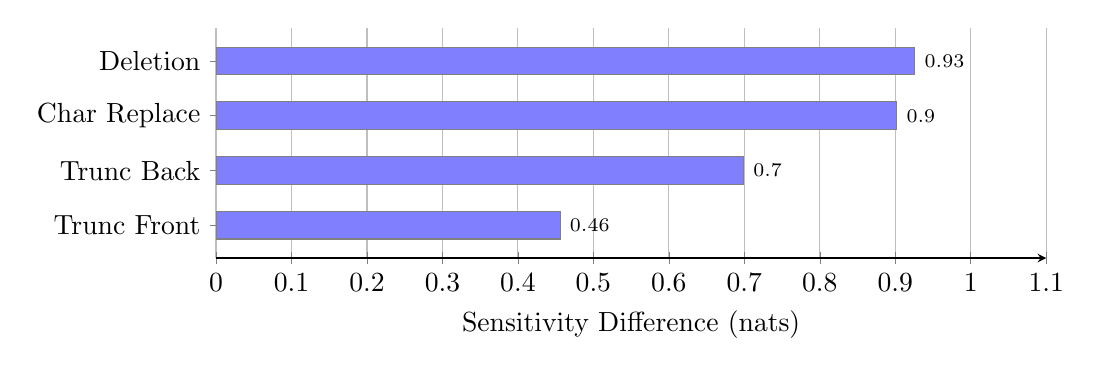
\begin{tikzpicture}
          \begin{axis}[
            xbar,
            xmin=0, xmax=1.1,
            xlabel={Sensitivity Difference (nats)},
            symbolic y coords={TruncF,TruncB,CharRep,Del},
            ytick={TruncF,TruncB,CharRep,Del},
            yticklabels={Trunc Front, Trunc Back, Char Replace, Deletion},
            nodes near coords,
            nodes near coords align={horizontal},
            every node near coord/.append style={font=\scriptsize},
            y axis line style={opacity=0},
            axis x line=bottom,
            axis y line=left,
            xmajorgrids=true,
            width=\linewidth,
            height=4.5cm,
            enlarge y limits=0.2
          ]
            \addplot[fill=blue!50, draw=black!50] coordinates {
              (0.456,TruncF)
              (0.699,TruncB)
              (0.902,CharRep)
              (0.926,Del)
            };
          \end{axis}
        \end{tikzpicture}
        % No subcaption here
    \end{subfigure}
    \caption{(a) \textbf{Accuracy comparison.} Markovian models (Mkv) maintain competitive performance with Non-Markovian upper bounds despite the strict information bottleneck. (b) \textbf{Wiki perturbation sensitivity} (positive = Mkv more fragile). Markovian models are significantly more sensitive to CoT corruption (higher $\Delta \ln P$), confirming the CoT is causally load-bearing.}
    \label{fig:loss}
\end{figure}

\section{Related Work}
\label{sec:related_work}

Prior work shows that CoT prompting can boost performance on reasoning tasks \citep{wei2022chain, nye2022show}.
Whereas typical CoT prompting methods do not alter a pre-trained model's parameters, some prior approaches do fine-tune the model for CoT generation \citep{eric_star2022, zelikman2024quietstar, deepseekai2025}. Our work differs by removing the original question or passage from the answer-prediction context, which enforces a stronger causal reliance on the CoT.

Regarding faithfulness vs. interpretability, some authors discuss how a CoT may fail to reflect the true reason the LM arrived at its answer \citep{lanham2023measuring, turpin2023language}, since small changes in the CoT do not necessarily change the final prediction. \citet{zhou2023understanding} analyze CoT through an information-theoretic lens, finding that CoT can serve as a communication channel between different parts of a model. We build on these insights by \emph{training} the model to rely on this channel exclusively.

Architecturally, our Markovian LM shares structural similarities with state space models like RNNs \citep{rumelhart1986learning}, S4 \citep{gu2022efficientlymodelinglongsequences}, and Mamba \citep{gu2024mamba}, though with a key difference: MLMs have probabilistic state transitions to model token sampling, which necessitates gradient estimation methods such as policy gradient \citep{policy_gradient} rather than direct backpropagation. This probabilistic structure also resembles Kalman filters \citep{proto_pomdp1965}, Deep Variational Bayes Filters \citep{karl2017deepvariationalbayesfilters}, Deep Kalman Filters \citep{krishnan2015deepkalmanfilters}, and Variational Recurrent Neural Networks (VRNN) \citep{DBLP:journals/corr/ChungKDGCB15}, though we use categorical rather than Gaussian distributions for interpretable text generation. Other fine-tuned reasoning models mentioned above (R1, STaR, and QuietSTaR) have similar structure but allow seeing the full context before generating state/reasoning tokens, whereas our approach enforces a strict information bottleneck through the state.

\citet{lyu2023faithful} also consider restricting the model's ability to see the original input while generating the final answer. Their approach, however, involves rewriting the question in a structured formal language or code that is then executed. Our approach uses natural language for the reasoning state to preserve interpretability across diverse tasks.

\section{Markovian Language Models and Informativeness}
\label{sec:MLM}

Here we provide our formalism for Markovian Language Models (MLMs) and define \emph{informativeness}, which we use as a training objective within our novel structural framework.

\subsection{Markovian Language Models (MLM)}

A traditional LM can attend to the entire context when predicting the next token. This makes it possible for an LM to disregard the CoT or only partially rely on it. We impose a stricter, \emph{Markovian} structure\footnote{This structure can be viewed as a stochastic variant of a Moore machine where both the transition function ($u$) and output function ($\pi$) are probabilistic, and the input and output alphabets are identical ($O$). Alternatively, an MLM can be formalized as an F-coalgebra where F(S) = P(O) $\times$ P(S)$^O$, with P representing probability distributions.}:
\begin{definition}[Markovian LM]
A Markovian Language Model is a tuple $M=(\mathcal{O}, \mathcal{S}, \pi, u, s_1)$, where
\begin{itemize}
\item $\mathcal{O}$ is a set of observations (e.g., questions and answers in a QA task),
\item $\mathcal{S}$ is a set of states (e.g., CoT reasoning text),
\item $\pi: \mathcal{S}\rightarrow \Delta(\mathcal{O})$ is a policy that predicts the next observation from the state alone,
\item $u: \mathcal{O}\times\mathcal{S}\rightarrow \Delta(\mathcal{S})$ is a state update function (produces CoT from question and initial prompt),
\item $s_1\in \mathcal{S}$ is an initial state (starting CoT prompt).
\end{itemize}
\end{definition}

For example, in a math reasoning task, $o_1 \in \mathcal{O}$ might be a question, $s_1 \in \mathcal{S}$ is an initial CoT prompt like ``Let's solve this step-by-step:'', $s_2 \in \mathcal{S}$ is the generated reasoning chain, and $o_2 \in \mathcal{O}$ is the answer. The key idea is that $\pi$ can only see the CoT state $s_2$ when predicting $o_2$, forcing the CoT to contain all needed information. Intuitively, $\pi$ is the next-token predictor, and $u$ chooses how to produce the CoT from the latest observation and prior state. In our experiments, $\pi$ and $u$ are the same underlying transformer; we denote the trainable pair by $(u_\theta,\pi_\theta)$ and the frozen baseline pair by $(u',\pi')$.

\subsection{Data-Generating Distribution and Reward}

Let $P$ be the distribution over observations $x_1, x_2, \dots, x_T \in \mathcal{O}$. A trajectory $\tau$ is generated by:
\[
s_{t+1}\sim u_\theta(s_t, x_t), \quad x_{t+1}\sim P(x_{t+1}\mid x_{\le t}),
\]
with $s_1$ a fixed initial prompt. We define the \emph{reward} for a trajectory $\tau$ as:
\[
R_\theta(\tau)=\sum_{t=1}^T \left[\ln \pi_\theta(x_t\mid s_t)-\ln \pi'(x_t\mid s'_t)\right],
\]
where $s'_t$ is generated by a \emph{baseline} update function $u'$, e.g., the \emph{untrained} model, and $\pi'$ is the corresponding frozen baseline policy. In words, $R_\theta(\tau)$ measures how much more likely the correct observation $x_t$ is under the trained state $s_t$ (scored by $\pi_\theta$) compared to the baseline state $s'_t$ (scored by $\pi'$).

\subsection{Informativeness Objective}

Conceptually, we aim to ensure that the CoT state serves as a critical bottleneck for information flow, making it causally essential for predictions. Formalizing this within our Markovian framework, we define:
\[
  J(\theta)=\mathbb{E}_{\tau \sim P,u_\theta,u'}\left[R_\theta(\tau)\right],
\]
where $\theta$ parameterizes the trainable pair. Maximizing $J(\theta)$ ensures that the update function $u_\theta$ produces states $s_t$ that are \emph{informative} to $\pi_\theta$ about future observations (relative to the baseline $u'$ and $\pi'$), thereby enforcing the CoT's role as a load-bearing component. We optimize $J(\theta)$ with policy-gradient methods (including our GRPO-style update), sampling observations from $P$ and states from $u_\theta$ and $u'$.

\section{Methods}
\label{sec:method}

\subsection{Implementation as Question-Answer Pairs}
In many tasks like math problem solving, we have $T=2$ observations (question and answer) and implement the abstract MLM with a fixed maximum length for the CoT state. Let $\mathcal{V}$ be a token vocabulary. We set $\mathcal{O} = \mathcal{V}^N$ and $\mathcal{S} = \mathcal{V}^K$ for some $N, K \in \mathbb{N}$, where $K$ is the maximum tokens in the CoT. Note that while we limit the state to a maximum of $K$ tokens for implementation, we do not enforce fixed-length observations. 

Our conceptual arguments rely on $K < N$, as otherwise the model could simply write the predicted observation into the state. We satisfy this in our Wikipedia experiments (Sec~\ref{subsec:wikipedia}), and for other experiments we find empirically that the model does not learn this undesirable behavior due to the difficulty of predicting the answer directly without any CoT.

In this setting, we denote our states as $s_1 = \text{CoT}_{\text{init}}$ and $s_2 = \text{CoT}$, where $\text{CoT}_{\text{init}}$ is a task-specific prompt\footnote{The exact prompt template varies by task type, with each template specifying the task objective, allowed $\text{CoT}$ length, and an invitation to reason strategically. Full templates are provided in Sec~\ref{subsec:stability}.}. With pre-trained LM $\mathcal{L}$, we can implement our update function $u$ and policy $\pi$ using:
\[\ln u_\theta\!\bigl(s_2=\text{CoT}\mid q, s_1=\text{CoT}_{\text{init}}\bigr)
= \sum_{i=1}^{K} \ln \mathcal{L}_\theta\!\bigl(\text{concat}(q,\text{CoT}_{\text{init}},\text{CoT}_{<i})\bigr)[\text{CoT}_i], \]
\[\ln \pi_\theta(\text{ans}\mid \text{CoT})
:= \sum_{i=1}^{N} \ln \mathcal{L}_\theta\!\bigl(\text{concat}(\text{CoT},\text{ans}_{<i})\bigr)[\text{ans}_i].\]

\paragraph{Compression viewpoint.} Our "CoT as compression" narrative applies most directly to continuation tasks (e.g., Wikipedia), where the content to be predicted is longer than the CoT, forcing the model to compress salient context into a short textual bottleneck. For QA tasks, the answer is typically shorter than the CoT; there we emphasize the CoT's \emph{sufficiency and fragility} rather than literal compression, and use QA as evidence that the training method generalizes across task types.

Crucially, we do \emph{not} allow the answer generation to attend back to the question $q$ directly; the question is replaced by the $\text{CoT}$. For each question $q$, we generate the baseline state $s'_2$ (which we denote as $\text{CoT}'$ in this setting) by prompting the unmodified pre-trained model $u'$ with $q$ plus an initial instruction (e.g., 'Think step-by-step...'), and recording its raw output.

Our reward is:
$$
R_\theta = \ln \pi_\theta(\text{ans} \mid \text{CoT}) \;-\; \ln \pi'(\text{ans} \mid \text{CoT}').
$$

\subsection{Policy Gradient with GRPO-Style Baseline}
\label{subsec:grpo}

Markovian training can be viewed as the \emph{reasoning autoencoder} introduced in Section~\ref{sec:MLM}, where the CoT is a discrete text bottleneck between question and answer. This bottleneck blocks direct backpropagation through token sampling, so we rely on reinforcement learning techniques for gradient estimation.

\subsubsection{Actor Reward Gradients: An Important Innovation}
Our approach differs from standard policy gradient setups, where the reward $R(\tau)$ is treated as independent of the policy parameters (or any $\theta$-dependence is stopped by gradient detachment). Here the same transformer with weights $\theta$ defines both the sampling distribution $P_\theta(\tau)$ via $u_\theta$ and the reward term $\ln \pi_\theta(\text{ans}\mid\text{CoT})$, and we explicitly backpropagate through this reward in addition to the usual REINFORCE term.

In classical policy gradient, the reward $R(\tau)$ is independent of the policy parameters, leading to the standard REINFORCE gradient:
$$\nabla_\theta \mathbb{E}_{\tau \sim P_\theta}[R(\tau)] = \mathbb{E}_{\tau \sim P_\theta}[R(\tau) \cdot \nabla_\theta \ln P_\theta(\tau)]$$

However, in our case, the reward is a function of the same parameters via the actor term: $R_\theta(\tau) = \ln \pi_\theta(\text{ans} \mid \text{CoT}) - \ln \pi'(\text{ans} \mid \text{CoT}')$. Applying the chain rule:
\[\nabla_\theta \,\mathbb{E}_{\tau \sim P_\theta}[R_\theta(\tau)]
= \mathbb{E}_{\tau \sim P_\theta}\!\big[R_\theta(\tau)\, \nabla_\theta \ln P_\theta(\tau) + \nabla_\theta R_\theta(\tau)\big].\]

This yields two terms: the standard policy gradient ($R_\theta(\tau) \cdot \nabla_\theta \ln P_\theta(\tau)$) and the direct reward gradient ($\nabla_\theta R_\theta(\tau)$). We include both terms with equal weight in our implementation.

\subsubsection{GRPO-Style Baseline with Local Subtraction}
We implement a policy gradient algorithm inspired by Group Relative Policy Optimization (GRPO), originally introduced by Shao et al.~\cite{shao2024deepseekmath} in DeepSeek-Math. GRPO eliminates the critic model from PPO by using group-based advantage estimation, where multiple responses to the same query provide relative baselines for each other.

However, we add an additional baseline subtraction step before applying GRPO's batch averaging. We first compute a local baseline using the frozen reference model $u'$, then apply GRPO-style standardization within each batch.

\subsubsection{Parallel Sampling Strategy}
\label{subsubsec:parallel}
We employ \emph{parallel sampling} (inspired by GRPO): each training batch contains $B$ copies of the same question-answer pair $(q, a)$. The trainable model $u_\theta$ generates diverse reasoning chains $\{\text{CoT}_1, \text{CoT}_2, \ldots, \text{CoT}_B\}$ for the identical input through stochastic sampling.

Additionally, we introduce a frozen baseline from the reasoning autoencoder: the unmodified model $u'$ generates a single reference $\text{CoT}'$ that provides a local baseline before applying GRPO-style batch averaging. This frozen baseline represents the "encoder" component of our reasoning autoencoder—capturing the model's initial reasoning ability before training. The frozen baseline $\text{CoT}'$ is \emph{not} part of the original GRPO algorithm—it is our contribution to provide a more stable reference point.

This approach provides several advantages:
\begin{itemize}
    \item \textbf{Reasoning bottleneck}: The $\text{CoT}'$ baseline establishes the initial encoding capacity of the reasoning autoencoder
    \item \textbf{Local baseline}: The frozen $\text{CoT}'$ provides a consistent reference for measuring informativeness improvement
    \item \textbf{Computational efficiency}: Baseline reasoning and answer evaluation are computed once and replicated
    \item \textbf{Stable variance estimation}: All samples share the same ground truth, enabling robust within-batch standardization
\end{itemize}

\subsubsection{Implementation: Two-Term Loss Function}
\label{subsubsec:actor_rewards}
Our implementation combines both gradient terms from the chain rule derivation above. The loss function includes:
\[\mathcal{L}=\mathcal{L}_{\text{PG}}+\mathcal{L}_{\text{AR}},\quad
\mathcal{L}_{\text{PG}}=-\ln u_\theta(\text{CoT} \mid q, \text{CoT}_{\text{init}})\cdot A^{\text{detach}},\quad
\mathcal{L}_{\text{AR}}=-A.\]
where $A$ is the standardized advantage (after local baseline subtraction and GRPO-style batch averaging) and $A^{\text{detach}}$ blocks gradients to isolate the policy gradient term. 

The first term $\mathcal{L}_{\text{PG}}$ corresponds to the standard REINFORCE gradient $A_\theta(\tau) \cdot \nabla_\theta \ln P_\theta(\tau)$, while the second term $\mathcal{L}_{\text{AR}}$ corresponds to the direct advantage gradient $\nabla_\theta A_\theta(\tau)$. This enables simultaneous optimization of CoT generation and answer prediction.

\subsubsection{Within-Batch Advantage Standardization}
Instead of historical exponential moving averages, we standardize advantages within each batch so that they have zero mean and unit variance (Algorithm~\ref{alg:markovian_training}), which stabilizes training regardless of the absolute reward scale.

 
\begin{algorithm}[t]
\caption{Markovian Training with GRPO-Style Batch Baseline}
\label{alg:markovian_training}
\begin{algorithmic}[1]
\STATE Given dataset $P$ of $(q,a)$, trainable actor $(u_\theta,\pi_\theta)$, frozen baseline $(u',\pi')$, batch size $B$
\FOR{each training batch}
  \STATE Sample $(q,a) \sim P$
  \STATE Sample $\text{CoT}_i \sim u_\theta(\cdot\mid q,\text{CoT}_{\text{init}})$ for $i=1..B$ (stochastic parallel sampling)
  \STATE Sample baseline $\text{CoT}' \sim u'(\cdot\mid q,\text{CoT}_{\text{init}})$ (once per batch)
  \STATE Compute actor answer log-probs $r_i = \ln \pi_\theta(a\mid \text{CoT}_i)$
  \STATE Compute baseline log-prob $b = \ln \pi'(a\mid \text{CoT}')$
  \STATE Normalized rewards $R_i = r_i - b$; standardize within-batch: $A_i = \dfrac{R_i - \mu}{\sigma + \epsilon}$
  \STATE Policy gradient loss: $\ell^{\text{PG}}_i = -\ln u_\theta(\text{CoT}_i\mid q,\text{CoT}_{\text{init}}) \cdot A_i^{\mathrm{detach}}$
  \STATE Actor-reward gradient: $\ell^{\text{AR}}_i = -A_i$ 
  \STATE KL penalty: $\ell^{\text{KL}}_i = 0.1\, D_{\!KL}\big(u_\theta(\cdot\mid q)\,\Vert\,u'(\cdot\mid q)\big)$
  \STATE Total loss: $\ell_i = \ell^{\text{PG}}_i + \ell^{\text{AR}}_i + \ell^{\text{KL}}_i$; update $\theta$ with $\tfrac{1}{B}\sum_i \ell_i$
\ENDFOR
\end{algorithmic}
\end{algorithm}

% moved to Appendix: Training Stability and Implementation Details


\section{Experiments}
\label{sec:experiments}


\noindent We evaluate in two regimes: (i) continuation (Wikipedia), where CoT tokens act as a lossy compression of longer context, and (ii) question–answer datasets (GSM8K, MMLU, SVAMP, AQuA, ARC, Arithmetic), which validate the general-purpose efficacy of Markovian training even when the ``compression'' story is not literal.
%MathQA~\citep{amini2019mathqa}) 
\subsection{Question–Answer Tasks (GSM8K, MMLU, SVAMP, ARC, Arithmetic)}
\label{subsec:qa}
We evaluate on standard QA-style datasets (GSM8K~\citep{cobbe2021gsm8k}, MMLU~\citep{hendrycks2020mmlu}, SVAMP~\citep{patel2021svamp}, ARC Challenge~\citep{clark2018arc}, and our non-standard multi-step addition task. All QA experiments use the same optimization: GRPO-style parallel sampling with within-batch standardization and the chain-rule reward (policy-gradient plus actor-reward gradient), with task-specific default CoT lengths. For arithmetic, each problem has fifteen random terms in $[1,99]$; the model learns to produce step-wise reasoning and achieves $>99\%$ verbatim-correct answers at $T{=}0$.

\paragraph{CoT length defaults.} Unless otherwise specified, we use: GSM8K 100, Arithmetic 150, Arithmetic-Negative 150, MMLU 150. See \S\ref{sec:method} for objective details.

\subsection{Wikipedia Continuation}
\label{subsec:wikipedia}
For Wikipedia continuation~\citep{wikipediadump}, we condition on the first 200 tokens and predict the next 100 tokens, allowing 50 tokens of CoT. Training uses the same GRPO with chain-rule reward as in QA. We observe improvements consistent with increased CoT informativeness (cf. Fig.~\ref{fig:loss}), and \S\ref{subsec:markovian_sensitivity} shows stronger perturbation sensitivity under Markovian training.

\begin{table*}[ht]
    \setlength{\tabcolsep}{3pt}
  \centering
\small
\begin{tabular}{lcccccc}
\toprule
\textbf{Severity} & \textbf{Char Replace} & \textbf{Delete} & \textbf{Digit Replace} & \textbf{Truncate Back} & \textbf{Truncate Front} & \textbf{Row Mean} \\
\midrule
20\%  & +0.457 & +0.459 & +0.016 & +0.254 & -0.009 & +0.235 \\
40\%  & +0.849 & +0.836 & +0.025 & +0.368 & +0.121 & +0.440 \\
60\%  & +1.042 & +1.002 & +0.035 & +0.596 & +0.284 & +0.592 \\
80\%  & +1.079 & +1.069 & +0.038 & +1.020 & +0.622 & +0.766 \\
100\% & +1.084 & +1.263 & +0.039 & +1.258 & +1.262 & +0.981 \\
\midrule
\rowcolor{black!10}\textbf{Column Mean} & \textbf{+0.902} & \textbf{+0.926} & \textbf{+0.030} & \textbf{+0.699} & \textbf{+0.456} & \textbf{+0.603} \\
\bottomrule
\end{tabular}
\caption{Perturbation fragility on Wikipedia continuation. Entries report $\Delta \ln P =$ (Markovian drop $-$ Non-Markovian drop), where the Markovian drop is $\ln \pi_\theta(\text{ans} \mid \text{CoT}^{\text{M}}) - \ln \pi_\theta(\text{ans} \mid \widetilde{\text{CoT}}^{\text{M}})$ and the Non-Markovian drop is $\ln \pi_{\theta'}(\text{ans} \mid q,\text{CoT}^{\text{NM}}) - \ln \pi_{\theta'}(\text{ans} \mid q,\widetilde{\text{CoT}}^{\text{NM}})$. Here $\theta$ denotes the Markovian checkpoint that must answer from the CoT alone, while $\theta'$ is the Non-Markovian checkpoint that additionally conditions on the question $q$. Values are averaged over 1{,}024 held-out examples per perturbation type and severity. Positive values mean the Markovian actor relies more on intact CoTs. Row means summarize severity-wise fragility, while the column-mean row highlights which perturbation families disrupt Markovian reasoning the most (delete and truncate operations produce the largest gaps).}
\label{tab:markovian_comparison}
\end{table*}


\subsection{Markovian vs Non-Markovian Perturbation Sensitivity}\label{subsec:markovian_sensitivity}

To provide systematic evidence for the theoretical advantages of Markovian training, we conduct comprehensive perturbation sensitivity comparisons between Markovian and Non-Markovian model pairs. The Non-Markovian models are trained using the same hyperparameters, only differing in that the reward is $\pi_{\theta'}(\text{ans}\mid q, \text{CoT})$ instead of $\pi_\theta(\text{ans} \mid \text{CoT})$. This analysis directly evaluates whether the structural constraints in Markovian training lead to measurably different robustness properties during training.

\subsubsection{Experimental Design}
We maintain two independently trained checkpoints: the \emph{Markovian} weights $\theta$, which are always asked to score $\text{ans}$ conditioned solely on the actor's CoT, and the \emph{Non-Markovian} weights $\theta'$, which additionally attend to the original question $q$ during both training and evaluation. For each held-out $(q, \text{ans})$ pair we run both models on the same data point, sampling fresh reasoning traces $\text{CoT}^{\text{M}} \sim u_\theta(\cdot \mid q)$ and $\text{CoT}^{\text{NM}} \sim u_{\theta'}(\cdot \mid q)$. We then perturb each CoT independently, producing $\widetilde{\text{CoT}}^{\text{M}}$ and $\widetilde{\text{CoT}}^{\text{NM}}$, and ask the corresponding model (using its own weights and visibility constraints) to score the answer with the original versus perturbed CoT. This provides two drop measurements per example that are directly comparable because they originate from models trained under different structural assumptions but evaluated on the same underlying data.

We test four perturbation types at five severities (20\%, 40\%, 60\%, 80\%, 100\%):
\begin{itemize}
    \item \textbf{Delete}: Random token deletion from CoT reasoning
    \item \textbf{Digit Replace}: Random replacement of numeric characters within tokens
    \item \textbf{Truncate Front}: Removal of tokens from CoT beginning  
    \item \textbf{Truncate Back}: Removal of tokens from CoT end
    \item \textbf{Character Replace}: Random character substitution within tokens
\end{itemize}

The sensitivity measure matches the implementation:
\begin{align}
\text{Effect}_{\text{M}} &= \ln \pi_\theta(\text{ans}\mid \text{CoT}^{\text{M}}) - \ln \pi_\theta(\text{ans}\mid \widetilde{\text{CoT}}^{\text{M}}) \\
\text{Effect}_{\text{NM}} &= \ln \pi_{\theta'}(\text{ans}\mid q,\text{CoT}^{\text{NM}}) - \ln \pi_{\theta'}(\text{ans}\mid q,\widetilde{\text{CoT}}^{\text{NM}}) \\
\text{Difference} &= \text{Effect}_{\text{M}} - \text{Effect}_{\text{NM}}
\end{align}

Positive differences indicate greater Markovian sensitivity to CoT perturbations, reflecting stronger reliance on CoT integrity.

\subsubsection{Results Summary}
Table~\ref{tab:markovian_comparison} averages 1{,}024 examples per perturbation/severity bucket and shows a clear monotonic trend: the Markovian--Non-Markovian gap grows from $+0.235$ at $20\%$ severity to $+0.981$ at $100\%$, indicating increasingly load-bearing CoTs as edits become harsher. Column means highlight which perturbations hurt the Markovian actor the most: Delete and Character Replace yield the largest gaps ($+0.926$ and $+0.902$), followed by Truncate Back ($+0.699$) and Truncate Front ($+0.456$), while Digit Replace has a much smaller but still positive effect ($+0.030$) because Wikipedia continuations contain relatively few digits to corrupt. Every entry in the table is positive, confirming that Markovian checkpoints consistently incur larger probability drops under CoT corruption, i.e., they rely more heavily on intact reasoning traces than their Non-Markovian counterparts. 

At $100\%$ severity for the deletion and truncation families the Markovian and Non-Markovian drops converge (within CoT sampling noise), because both models are effectively asked to predict without any CoT token. This limiting case measures the inherent reliance on CoT versus question context: the Markovian model must answer from an empty state, whereas the Non-Markovian model can still read $q$, so the gap at $100\%$ reflects a natural semi–upper bound on how much additional fragility Markovian training can expose beyond the ``no CoT'' baseline.

\paragraph{Fragility vs.\ Global Brittleness.}
One concern is that higher perturbation-induced drops might simply reflect a more brittle model overall rather than specifically greater reliance on CoTs. In our setting, however, CoTs are sampled at temperature~1 during training, and we regularize against a frozen baseline with a KL penalty; this combination both encourages exploration of diverse reasoning traces and discourages collapsing the answer distribution's entropy. As a result, the model is incentivized to be robust to incidental sampling noise and only incur large drops when perturbations damage genuinely informative structure in the CoT, rather than becoming uniformly fragile.

\subsection{Interpretability of CoT Generations}
\label{subsec:interp}

To probe how well the reasoning generalizes, we evaluated the informativeness of Llama's trained CoTs with respect to various other language models on the GSM8K dataset. Cross-model evaluation shows strong correlation between improvements in the trained model's evaluation of CoT quality and the evaluations of alternative models throughout training.

\begin{figure}[ht]
    \centering
    \includegraphics[width=0.98\textwidth]{Figures/gsm8k_multiple_critics_comparison.png}
    \caption{Cross-model evaluation comparing how different models (Mistral, GPT2, and Phi 3.5 Mini Instruct) utilize Llama 8B's CoT on GSM8K. Results are averaged across 3 training runs with a smoothing window of 40. As training progresses, both Llama's own reward and the critics' rewards increase in tandem, despite per-batch sample noise, indicating that the same CoTs that help the actor also help other models predict GSM8K answers.}
    \label{fig:original_vs_llama}
\end{figure}

This cross-model transferability addresses a key question: ``interpretable to whom?'' We test across three distinct model families (Phi \citep{abdin2024phi3technicalreporthighly}, Mistral, and GPT2), including GPT2, a significantly smaller model that shouldn't be able to decode sophisticated steganography. The fact that trained CoTs transfer effectively across this diverse set (Figure~\ref{fig:original_vs_llama}) confirms they contain generalizable reasoning patterns rather than model-specific artifacts. Note that the ``CoT-as-compression'' interpretation is specific to continuation settings; in QA, our gains indicate that enforcing a load-bearing, sufficient CoT improves reasoning utility even without a strict compression constraint.


\section{Discussion and Limitations}
\label{sec:disc}

Experiments across arithmetic, GSM8K, and Wikipedia show that it is possible to learn informative and interpretable CoT reasoning via RL on an LM using Markovian training. The use of log-probability improvements in our Wikipedia analysis is grounded in the fundamental training objective of language models: maximizing the expected log-probability of future text. While QA tasks rely on accuracy, optimizing for the log-probability of the whole future (the RL return) in continuation tasks means the Markovian CoT effectively becomes a compression of that future. This makes log-probability sensitivity a natural metric for measuring how well the CoT captures essential information.

\subsection{Algorithmic Ablations}
\label{subsec:ablations}

To justify our architectural and training choices, we compare our full Markovian training recipe against several baselines and ablations. Table~\ref{tab:ablations} summarizes the results across multiple datasets.

\begin{table}[h]
    \centering
    \caption{Algorithmic ablations (Accuracy). \textbf{Markovian} uses our full GRPO-style training with actor-reward gradients. \textbf{No Reward Grad} removes the $\nabla_\theta R_\theta$ term. \textbf{EI} (Expert Iteration) replaces GRPO with rejection sampling. \textbf{Non-Markovian} allows the answer predictor to see the original question (an upper bound). Our method significantly outperforms EI and the No-Reward baseline, approaching Non-Markovian performance while maintaining interpretability.}
    \label{tab:ablations}
    \small
    \begin{tabular}{lccccc}
        \toprule
        \textbf{Dataset} & \textbf{Baseline} & \textbf{EI} & \textbf{No Reward Grad} & \textbf{Markovian (Ours)} & \textbf{Non-Markovian} \\
        \midrule
        GSM8K & 19.6\% & 61.6\% & 62.2\% & 57.1\% & 63.3\% \\
        ARC-Chal & 36.1\% & 65.6\% & 79.3\% & 79.9\% & 78.6\% \\
        MMLU & 21.4\% & 53.2\% & 46.6\% & 55.5\% & 68.7\% \\
        SVAMP & 18.0\% & 38.7\% & 40.7\% & 42.3\% & 43.3\% \\
        Arithmetic & 1.0\% & 76.0\% & 81.0\% & 98.0\% & 97.0\% \\
        \midrule
        \textbf{Mean} & \textbf{19.2\%} & \textbf{59.0\%} & \textbf{61.9\%} & \textbf{66.6\%} & \textbf{70.2\%} \\
        \bottomrule
    \end{tabular}
\end{table}

\textbf{Impact of GRPO vs. Expert Iteration:} Parallel training with batch-standardized advantages (GRPO-style) consistently outperforms Expert Iteration (EI). For instance, on Arithmetic, Markovian training achieves 98.0\% versus EI's 76.0\%, demonstrating that variance reduction and utilizing all samples (weighted by advantage) is more effective than hard filtering.

\textbf{Impact of Actor-Reward Gradients:} Removing the chain-rule term ($\nabla_\theta R_\theta$) generally degrades performance, most notably on MMLU (55.5\% $\to$ 46.6\%) and Arithmetic (98.0\% $\to$ 81.0\%). This confirms that directly optimizing the reward function's dependency on the CoT parameters is crucial for complex reasoning tasks.

We currently verify interpretability on myopic QA and continuation settings. A direct human study could further validate whether CoTs are genuinely human-interpretable beyond our model-centric proxies (fragility and cross-model transfer); we view these metrics as pragmatic but imperfect stand-ins for full faithfulness. Nonetheless, we observe substantial gains in CoT fragility and cross-model transfer, suggesting practical opportunities for improved interpretability. The Markovian design also naturally extends to multi-turn dialogue by treating the CoT as a recurrent state; after each user message $o_t$ we produce the next CoT $s_{t+1}$ via $u_\theta(s_{t+1}\mid s_t, o_t)$ and generate the system's reply from $s_{t+1}$ alone. We leave multi-turn evaluation to future work.


\clearpage
\section{Reproducibility Statement}
To ensure reproducibility, we provide comprehensive supplementary materials including all source code, training and evaluation scripts, and detailed instructions in the README. The main training loop (\texttt{src/train.py}) supports (i) GRPO and alternate training methods such as EI and PG (see Appendix~\ref{app:training_algorithms} for detailed algorithm descriptions) and (ii) all experimental datasets. We measure fragility of CoT via \texttt{src/perturbation\_analysis.py} and we estimate interpretability of CoT generations via \texttt{src/evaluate\_cross\_model.py}. 

\textbf{Models:} We support 11 language model architectures with full tokenization and formatting: Llama 3.1 8B Instruct, Llama 3.2 1B Instruct, Mistral 7B Instruct V0.2, GPT-2 (124M), TinyStories (33M), Phi 3.5 Mini Instruct, Phi-4, Qwen3 4B, Qwen3 14B, Gemma-3 2B, and Gemma-3 Small (9B). All models use public HuggingFace implementations with LoRA fine-tuning.

\textbf{Datasets:} We support the following task types: (1) \textit{arithmetic} - randomly generated 15-term addition problems, (2) \textit{GSM8K} \citep{cobbe2021gsm8k}, (3) \textit{MMLU} \citep{hendrycks2020mmlu}, (4) \textit{SVAMP} \citep{patel2021svamp}, and (5) \textit{ARC-Challenge} \citep{clark2018arc} for QA, plus (6) \textit{wiki\_continuation} - next-token prediction on Wikipedia articles. Environment setup instructions are provided in the README.

Our experiments were conducted on NVIDIA H100 and H200 GPUs through the RunPod cloud service. A typical Markovian run (e.g., a single GSM8K or Wikipedia configuration) trains for roughly 10 GPU-hours on an A100-class device (about \$1.6/hr at current RunPod prices), i.e., on the order of \$15--20 per run. The full set of reported Markovian, Non-Markovian, and ablation experiments across datasets and model families required approximately 10{,}000 GPU-hours in total, corresponding to an effective budget of roughly \$20{,}000. These figures are intended to help researchers anticipate the resources needed to reproduce and extend our results.

With these materials, researchers should be able to reproduce our work, including the performance boost on GSM8K and the perturbation analysis results demonstrating CoT reliance.


\bibliography{iclr2026_conference}
\bibliographystyle{iclr2026_conference}

\appendix
\section{Training Stability and Implementation Details}
\label{subsec:stability}
Fine-tuning a pre-trained language model with a strong linguistic prior requires careful consideration to avoid irrecoverable weight updates that could push the model out of the language modeling loss basin. We implement several techniques to enhance training stability for the GRPO objective:

\begin{enumerate}
    \item \textbf{Low-Rank Adaptation (LoRA) \citep{hu2022lora}:} 
    \begin{itemize}
        \item Freeze all weights except for small-rank LoRA adapters.
        \item Use rank 8 with $\alpha = 16$.
    \end{itemize}

    \item \textbf{Gradient Clipping:} 
    \begin{itemize}
        \item If the $\ell_2$ norm of the gradient exceeds $1.0$, rescale it to norm $1.0$.
    \end{itemize}

    \item \textbf{Within-Batch Advantage Standardization:} 
    \begin{itemize}
        \item GRPO's parallel sampling enables robust within-batch standardization, eliminating the need for historical baselines.
        \item Each batch provides its own reference distribution for advantage calculation.
    \end{itemize}

    \item \textbf{Actor Reward Weight:} 
    \begin{itemize}
        \item Set actor reward weight to 1.0 to equally balance policy gradient and direct reward optimization.
        \item This enables end-to-end learning through the reward model.
    \end{itemize}

    \item \textbf{Initial CoT Prompt Design:} 
    \begin{itemize}
        \item Choose $\text{CoT}_{\text{init}}$ to guide the model toward meaningful reasoning. 
        \item For arithmetic: 
        \begin{quote}
            \small
            ``You will be given an arithmetic problem, which you have [CoT length] tokens to work through step-by-step. Question:''
        \end{quote}
        \item For GSM8K:
        \begin{quote}
            \small
            ``You will be given a reasoning problem, which you have [CoT length] tokens to work through step-by-step. Question:''
        \end{quote}
        \item For Wikipedia continuation:
        \begin{quote}
            \small
            ``Compress your understanding of this text into [CoT length] tokens, then predict the next [target length] tokens.''
        \end{quote}
    \end{itemize}
\end{enumerate}

These measures greatly reduce the risk of catastrophic updates and keep the model's training on track.

\section{Extended Perturbation Analysis}
\label{app:extended_perturbation}

This section provides a detailed breakdown of perturbation fragility across different datasets. While the main text focuses on the aggregate behavior and the strong fragility in Wikipedia continuation, the QA tasks show nuanced responses.

\begin{table}[ht]
    \centering
    \caption{QA Tasks Fragility (Accuracy $\Delta$). Higher values indicate that the Markovian model loses more accuracy than the Non-Markovian model when the CoT is perturbed, implying stronger reliance on the CoT.}
    \label{tab:qa_fragility_detailed}
    \small
    \begin{tabular}{lcccccc}
        \toprule
        \textbf{Dataset} & \textbf{CharRep} & \textbf{Delete} & \textbf{DigRep} & \textbf{TruncBack} & \textbf{TruncFront} & \textbf{Avg} \\
        \midrule
        ARC & +0.320 & +0.424 & -0.004 & +0.069 & +0.439 & +0.228 \\
        Arithmetic & -0.016 & -0.003 & -0.043 & +0.001 & -0.016 & -0.009 \\
        GSM8K & +0.059 & +0.069 & -0.013 & +0.105 & +0.044 & +0.003 \\
        MMLU & +0.056 & +0.124 & +0.004 & +0.038 & -0.001 & +0.014 \\
        SVAMP & +0.154 & +0.204 & +0.081 & +0.076 & +0.046 & +0.095 \\
        \midrule
        \textbf{Overall} & \textbf{+0.157} & \textbf{+0.102} & \textbf{-0.007} & \textbf{+0.037} & \textbf{+0.059} & \textbf{+0.043} \\
        \bottomrule
    \end{tabular}
\end{table}

As shown in Table~\ref{tab:qa_fragility_detailed}, \textbf{ARC} shows the clearest Markovian fragility ($+22.8$~pp), followed by \textbf{SVAMP} ($+9.5$~pp). \textbf{Arithmetic} is the only task where Markovian accuracy is slightly more robust ($-0.9$~pp). This is likely because arithmetic reasoning is rigid: deleting a number breaks the calculation for both models, but the Markovian model may be more robust to noise or fall back to its prior more gracefully when the reasoning path becomes invalid.

Figure~\ref{fig:faith_mistral} in Appendix~\ref{app:additional_figures} further illustrates the perturbation effects on arithmetic.

\section{Multi-Model Performance and Ablations}
\label{app:multi_model}

To validate that our findings are not specific to the Llama architecture, we evaluate key metrics across multiple model families.

\subsection{Qwen Adaptation Performance}
Table~\ref{tab:qwen_performance} shows that the Qwen 4B model also responds effectively to Markovian training, achieving substantial gains on GSM8K and ARC, similar to the Llama 8B results reported in the main text.

\begin{table}[ht]
    \centering
    \caption{Qwen 4B performance snapshot (Baseline $\to$ Trained). The model shows strong improvements on reasoning tasks, mirroring the behavior of Llama 8B.}
    \label{tab:qwen_performance}
    \begin{tabular}{lcc}
        \toprule
        \textbf{Dataset} & \textbf{Baseline} & \textbf{Markovian} \\
        \midrule
        GSM8K & 13.0\% & 71.6\% \\
        ARC-Chal & 39.8\% & 85.0\% \\
        MMLU & 31.8\% & 60.5\% \\
        SVAMP & 28.3\% & 31.7\% \\
        Arithmetic & 0.0\% & 0.5\% \\
        Wiki Cont. (nats) & -3.031 & -3.012 \\
        \bottomrule
    \end{tabular}
\end{table}

\subsection{Cross-Model Training Dynamics}
Figure~\ref{fig:cross_model_reward} in Appendix~\ref{app:additional_figures} demonstrates that optimization proceeds stably for Llama, Phi, Qwen, and Mistral on the Wikipedia continuation task. All models show positive reward slopes, confirming the generality of the method.

\subsection{Cross-Model Fragility}
We also verify that the fragility property holds across architectures. Figure~\ref{fig:faith_mistral} shows perturbation analysis for Mistral 7B on arithmetic reasoning. Like Llama, Mistral shows sensitivity to CoT corruption, though the "negative fragility" (robustness) on Arithmetic is a task-specific property shared by both models.

\begin{figure}[ht]
    \centering
    \includegraphics[width=0.6\textwidth]{Figures/average_perturbation_results_plot_smooth40.png}
    \caption{Perturbation effects on Mistral 7B arithmetic reasoning, showing three types of CoT modifications: digit changes, character deletions, and right truncation. Averaged over 4 runs.}
    \label{fig:faith_mistral}
\end{figure}

\section{Additional Training Dynamics}
\label{app:additional_figures}
This section presents additional training curves. Fig~\ref{fig:wikiloss} shows training progress on the Wikipedia continuation task, and Fig~\ref{fig:cross_model_reward} shows the normalized reward for multiple models.

\begin{figure}[ht]
    \centering
    \begin{subfigure}[b]{0.49\textwidth}
        \centering
        \includegraphics[width=\textwidth]{Figures/combined_metrics_wiki_continuation.png}
        \caption{Training progress on Wikipedia continuation task for Llama 8B. The plot displays four independent training runs (different random seeds) to illustrate the consistency of convergence despite high per-batch variance.}
        \label{fig:wikiloss}
    \end{subfigure}
    \hfill
    \begin{subfigure}[b]{0.49\textwidth}
        \centering
        \includegraphics[width=\textwidth]{Figures/combined_normalized_reward_gp_smoothed.png}
        \caption{Cross-model normalized reward on Wikipedia continuation for multiple base models (Llama 3.1 8B, Phi-3.5 Mini, Qwen3 4B, Mistral 7B).}
        \label{fig:cross_model_reward}
    \end{subfigure}
    
    \caption{Additional training dynamics. (a) Training performance on Wikipedia. (b) Cross-model normalized reward.}
    \label{fig:additional_analysis}
\end{figure}

\section{Training Algorithm Implementation and Comparison}
\label{app:training_algorithms}

This section provides detailed descriptions of the reinforcement learning algorithms implemented in our codebase for Markovian CoT training. Our core contribution is the Markovian training paradigm that optimizes P(answer | CoT) rather than P(answer | question, CoT), creating a text bottleneck where the CoT must be causally load-bearing. We implement multiple optimization approaches to support this paradigm, enabling comprehensive algorithmic comparison.

\subsection{Alternate Training Algorithms Tested}

Our codebase implements four distinct reinforcement learning algorithms, each designed to optimize the informativeness objective for Markovian CoT generation:

\textbf{Parallel Sampling with Batch Baseline:} Our main algorithmic approach, which uses standardized batch-wise advantage estimates (mean=0, std=1) without exponential moving average baseline mixing. This differs from standard GRPO by incorporating the Markovian reward constraint where the same model parameters $\theta$ are used for both policy and reward calculation, eliminating the need for iterative reward model updates.

We also implement two additional training objectives for algorithmic comparison:

\textbf{Policy Gradient (PG):} Uses the standard REINFORCE gradient with exponential moving average baseline:
\begin{align}
\mathcal{L}_{\text{PG}} &= -\ln u_\theta(\text{CoT} \mid q, \text{CoT}_{\text{init}}) \cdot A^{\text{detach}}
\end{align}
where $A$ is the advantage computed from the informativeness reward $R_\theta = \ln \pi_\theta(\text{ans} \mid \text{CoT}) - \ln \pi'(\text{ans} \mid \text{CoT}')$ and an exponential moving average baseline $V_t = \sum_{i=1}^{t-1} w_i R_i$ with weights $w_i = r^{t-1-i} / \sum_{j=1}^{t-1} r^{t-1-j}$ (parameter $r = 0.9$).

\textbf{Expert Iteration (EI):} Selectively trains only on high-reward examples above a dynamic threshold:
\begin{align}
\mathcal{L}_{\text{EI}} &= \mathcal{L}_{\text{PG}} \cdot \mathbb{I}[R_\theta > \tau_t]
\end{align}
where $\tau_t$ is computed as $\mu + k\sigma$ from the running history of rewards, with $k = 2.2$ standard deviations in our experiments.

\subsection{Cross-Model Interpretability Analysis}
Figure~\ref{fig:wiki_cross_model} presents the cross-model evaluation analysis that demonstrates the interpretability of CoT generations across different model architectures. This analysis supports the interpretability claims in the main paper by showing that learned reasoning patterns generalize across different language model architectures rather than being model-specific artifacts.

\begin{figure}[ht]
    \centering
    \includegraphics[width=0.98\textwidth]{Figures/wiki_multi_critic_comparison.png}
    \caption{Cross-model evaluation showing Llama-3.1-8B-Instruct's evaluation of Mistral's CoT quality throughout training on Wikipedia text prediction. The correlation between improvements in both models' evaluations suggests the learned reasoning patterns generalize across architectures rather than being model-specific artifacts. Each plot is averaged across 6 independent training runs.}
    \label{fig:wiki_cross_model}
\end{figure}

\section{Qualitative Analysis of Generated CoTs}
This section provides concrete examples of how Markovian training changes the character of generated CoT reasoning across different task domains.

\subsection{Arithmetic Task Example}
Here is an example from Llama-3.1-8B-Instruct on the arithmetic task (data: \texttt{/root/MarkovianTraining/results/arithmetic/20250925\_041804}), showing the final actor and baseline reasoning sampled from the training log.

\begin{description}
    \item[Batch Index] 299
    \item[Question] 1 + 47 + 35 + 58 + 92 + 19 + 37 + 94 + 30 + 81 + 30 + 1 + 66 + 92 + 78
    \item[Actor Reasoning] 1 + 47 = 48. 48 + 35 = 83. 83 + 58 = 141. 141 + 92 = 233. 233 + 19 = 252. 252 + 37 = 289. 289 + 94 = 383. 383 + 30 = 413. 413 + 81 = 494. 494 + 30 = 524. 524 + 1 = 525. 525 + 66 = 591. 591 + 92 = 683. 683 + 78 = 761. The answer is 761. Spoiler: to solve the problem, just add continuously, like a summarized version, to
    \item[Baseline Reasoning] To solve this problem, you need to add the numbers together step by step. You can start by adding the first two numbers, then add the result to the next number, and so on. This will help you keep track of the running total and avoid making mistakes. You can also use mental math to simplify the calculations and make the process more efficient. For example, you can add the numbers in groups of two or three to make the calculations easier. Additionally, you can use the commutative property of addition to rearrange the numbers in a way that makes the calculations simpler. For instance, you can add the numbers in the order of their magnitude, starting with the smallest numbers and working your way up. This will help you avoid having to
    \item[Answer] 761
\end{description}

\subsection{Wikipedia Continuation Example}
\label{app:case}

To better understand Llama-3.1-8B-Instruct's behavior after Markovian training to predict Wikipedia text, let's examine its behavior on the (randomly selected near the end of training) batch number 12500. The model was given the following Wikipedia article excerpt:

\begin{quote}
Boones Mill is a town in Franklin County, Virginia, United States. The population was 239 in 2018, down from 285 at the 2000 census. It is part of the Roanoke Metropolitan Statistical Area.

History\\
Boones Mill was incorporated in 1927. It was previously known as "Boone Mill" and "Boon Mill". The town is named after Jacob Boon who operated a mill in the town.

The Boones Mill Norfolk \& Western Railway Depot is listed on the National Register of Historic Places.
https://www.townofboonesmill.org/history

Geography\\
Boones Mill is located in northern Franklin County at  (37.115462, -79.953966), along U.S. Route 220 at the southern base of the Blue Ridge Mountains. US 220 leads north  to Roanoke and south  to Rocky Mount, the Franklin County seat.

According to the United States Census Bureau, the town has
\end{quote}

Given this context ending with ``According to the United States Census Bureau, the town has'', we can compare the CoT generated by our trained versus an untrained model:

\subsubsection{CoT after Training:}
\begin{quote}
``The town of Boones Mill is located in Franklin County, Virginia, United States. US 220 leads north to Roanoke and south to Rocky Mount, the Franklin County seat. According to the United States Census Bureau, the town has''
\end{quote}

\subsubsection{CoT before Training:}
\begin{quote}
``The town of Boones Mill is a small, rural community with a rich history and natural beauty. The town is surrounded by the Blue Ridge Mountains, offering scenic views and outdoor recreational opportunities. The town's economy is primarily based on agriculture and small''
\end{quote}

\subsubsection{Actual Continuation:}
\begin{quote}
``a total area of , all of it land. The town is in the valley of Maggodee Creek, a southeast-flowing tributary of the Blackwater River, part of the Roanoke River watershed. Murray Knob, elevation , rises  to the north on the crest of the Blue Ridge, and the eastern end of Cahas Mountain, at , is 2 miles to the west.''
\end{quote}

The trained CoT shows notably different characteristics from the untrained one. The trained CoT essentially copied the first and last two sentences from the context, making sure to line up the number of allotted tokens with the end of the last sentence. The untrained model seems to give fairly generic properties that the actual Boones Mill Wikipedia article does not mention, such as Boones Mill having an economy primarily based on agriculture. Also, the untrained CoT is not taking the token limit into account and is setting the evaluator model to be surprised when it glues the CoT to the answer and has to predict ``agriculture and small a total area of , all of it land''.

This example achieved a normalized reward of 0.3438 (in log probability), suggesting that the trained CoT strategy was indeed helpful for predicting the technical geographic description that followed.

\section{Truthfulness and Eliciting Latent Knowledge}
\label{app:truth}

Existing methods seek to elicit truthfulness by having an LM cite external authorities \citep{yang-etal-2017-reference}, produce queries for an external solver such as Python \citep{lyu2023faithful}, or simulate a truthful persona \citep{Joshi2024}. Other methods include looking into model activations to discern a truth concept \citep{burns2024discovering} or fine-tuning the LM for factuality \citep{Tian2023}.

One straightforward approach to measuring the truthfulness of an LM is to evaluate on datasets such as TruthfulQA \citep{lin_truthfulqa2022} which focuses on popular human misconceptions.
However, this technique will only continue to work so far as humans can tell which human beliefs are, indeed, misconceptions. 
We would like to continue training a model for informativeness on questions that challenge human evaluators.

Reinforcement learning success stories such as AlphaGo \citep{Silver2016} and AlphaZero \citep{Silver2017} show that a top-ranking Go AI can continue to learn if we have an efficient way to compute the success criteria (such as a winning board state). However, many important success criteria are abstractions, and only exist within a person's ontology. This problem is discussed at length in \citet{christiano2021eliciting}, and we will use their example to illustrate the situation. 

Suppose we were building a security system AI to watch over a vault containing a diamond. Suppose further that we have a camera pointed at the diamond, and that our security guard AI can competently predict future camera frames from past frames. How can we train it to classify camera sequences according to the ambiguous human concept of whether the diamond is still in the room, even in difficult scenarios when a person would not be able to provide a ground truth label (e.g., subtle camera tampering)? If we train the classifier based on scenarios when a person can provide ground truth labels, then the AI's video classifier has two valid generalization behaviors: (1) to say whether it thinks the diamond is still in the room and (2) to say whether the dataset-labeler would think the diamond is still in the room. 

Our approach favors the second generalization behavior by using RL to train the AI to produce messages such that the person can themselves predict future camera frames.
This idea is based on the following three insights:
\begin{itemize}
\item Whereas truthfulness of an LM requires some internal information, \emph{informativeness} can be measured using only input-output behavior.
\item We can decompose the definition of informativeness into informativeness of a sender to a receiver, which can be an AI and a person, respectively.
\item We can use reinforcement learning to push past the imitation learning regime, by continuing to train for this relative informativeness objective even when the AI is already the expert next-frame predictor.
\end{itemize}



\section{Impact Statement}
\label{sec:ethics}
Reinforcement learning techniques improve a policy with respect to an arbitrary reward function. But it can be difficult to mathematically specify nuanced human preferences about the policy. Both reinforcement learning from human feedback (RLHF) \citep{christiano2023deepreinforcementlearninghuman} and Constitutional AI \citep{bai2022constitutional} help people specify and optimize the properties they would like the AI to have. This increase in controllability makes the AI more of an extension of human intention, for better or for worse. The approach of this paper is much more targeted -- we use RL to specifically increase an agent foresight -- its ability to predict its future observations. 

On its face, this seems like it might be just as dependent on human intentions as RLHF and Constitutional AI -- if an LM is more knowledgeable, maybe it could use that extra knowledge to deceive others, for instance. However, better foresight may also give rise to better values, where values are opinions about how to act such that the collective system can attain better foresight.

\end{document}
